%%
%% Copyright 2007, 2008, 2009 Elsevier Ltd
%%
%% This file is part of the 'Elsarticle Bundle'.
%%

\documentclass[preprint,12pt,a4paper]{elsarticle}

\usepackage{amssymb}
\usepackage{hyperref}
\usepackage{graphicx}
\usepackage[utf8]{inputenc}
\usepackage[T1]{fontenc}
\usepackage{amsmath}
\usepackage{tikz}
\usetikzlibrary{shapes.geometric, arrows.meta, positioning, fit, backgrounds, calc}
\usepackage{float}
\usepackage{pifont}
\usepackage{listings}
\lstdefinelanguage{JavaScript}{
  keywords={async, await, const, let, var, function, return, if, else, for, while, do, switch, case, break, continue, new, try, catch, throw, typeof, instanceof, in, of, class, export, import, default, from, extends, super, this, true, false, null, undefined},
  morecomment=[l]{//},
  morecomment=[s]{/*}{*/},
  morestring=[b]',
  morestring=[b]",
  morestring=[b]`,
  sensitive=true
}
\lstset{
  basicstyle=\ttfamily\scriptsize,
  numbers=left,
  numberstyle=\tiny,
  numbersep=5pt,
  frame=single,
  breaklines=true,
  captionpos=b,
  tabsize=2,
  showstringspaces=false,
  columns=flexible
}
\setlength{\parindent}{0pt}

\journal{SoftwareX}

\begin{document}
\renewcommand{\labelenumii}{\arabic{enumi}.\arabic{enumii}}

\begin{frontmatter}

\title{Architecture of the Avalia+Tec Platform with Cryptographic Security for Transparent and Auditable Selection Processes}

\author[label1]{Luiz Diego Vidal Santos\corref{cor1}}
\author[label2]{Catuxe Varjão de Santana Oliveira}
\author[label4]{Dulce Paloma Vidal Santos}
\author[label1]{Tânia Cristina Azevedo}
\author[label3]{Renisson Neponuceno de Araújo Filho}
\author[label5]{Jémison Mattos dos Santos}
\author[label6]{Milton Marques Fernandes}
\author[label7]{Francisco Sandro Rodrigues Holanda}

\address[label1]{Universidade Estadual de Feira de Santana, Departamento de Ciências Exatas, Feira de Santana, Brasil}
\address[label2]{Universidade Federal de Sergipe, Programa de Pós-Graduação em Ciência da Propriedade Intelectual, São Cristóvão, Brasil}
\address[label3]{Universidade Federal Rural de Pernambuco, Departamento de Engenharia Rural, Recife, Brasil}
\address[label4]{Universidade Tiradentes, Departamento de Direito, Aracaju, Brasil}
\address[label5]{Universidade Estadual de Santa Cruz, Ilhéus, Brasil}
\address[label6]{Universidade Federal de Sergipe, Departamento de Ciências Florestais, São Cristóvão, Brasil}
\address[label7]{Universidade Federal de Sergipe, Departamento de Engenharia Agronômica, São Cristóvão, Brasil}

\ead{ldvidal@uefs.br}
\cortext[cor1]{Corresponding author}

\begin{abstract}
Selection processes in academic institutions and public organizations are frequently managed through email and spreadsheets, creating legal vulnerabilities, version-control errors, and data protection non-compliance. This paper presents avalia+Tec, an open-source SaaS platform that enforces cryptographic integrity verification (SHA-256), tamper-evident hash-chained audit trails with external RFC~3161 timestamp anchoring, and end-to-end traceability for selection workflows. The system operates through a responsive web portal for candidate submissions and administrative oversight, and an Electron-based desktop application for structured blind evaluation. A preliminary single-institution deployment at Universidade Estadual de Feira de Santana processing 60 submissions with 6 evaluators was associated with a 65\% reduction in review-to-decision cycle time (95\% CI: [55\%, 73\%], Mann--Whitney $U = 0$, $p = 0.029$, $r = 1.0$), no formal candidate disputes during the observation period, and a 45.4\% reduction in evaluator time per submission (95\% CI: [26\%, 59\%]). The platform provides technical controls supporting regulatory compliance with Brazil's LGPD. The scientific contribution resides not in novel cryptographic primitives but in the systematic integration engineering of well-established techniques to address a concrete, underserved institutional governance problem. avalia+Tec is freely available under the MIT License.
\end{abstract}

\begin{keyword}
selection processes \sep cryptographic audit trails \sep institutional governance \sep SaaS platform \sep SHA-256 integrity \sep LGPD compliance \sep open-source
\end{keyword}

\begin{highlights}
\item Auditable selection workflow using SHA-256 hashing and tamper-evident hash-chained logs.
\item HMAC-SHA256 signatures ensure integrity in blind peer-review scorecards.
\item Automation was associated with a 65\% reduction in administrative cycle time.
\item External RFC~3161 timestamp anchoring strengthens tamper-evidence beyond internal controls.
\item Technical controls supporting LGPD compliance via role-based data segregation and automatic PII redaction.
\end{highlights}

\end{frontmatter}

%% ============================================================
%% HIGHLIGHTS (submitted separately; included here for reference)
%% ============================================================
%% - Open-source SaaS platform with SHA-256 document integrity verification
%% - Immutable hash-chained audit trails for legally defensible selection processes
%% - Dual-frontend architecture: web portal (Vue.js) and desktop app (Electron)
%% - Initial deployment eliminated formal candidate disputes during observation period
%% - LGPD compliance via PII segregation, encryption-at-rest, and role-based access

\section*{Metadata}

\begin{table}[!h]
\begin{tabular}{|l|p{6.5cm}|p{6.5cm}|}
\hline
\textbf{Nr.} & \textbf{Code metadata description} & \textbf{Metadata} \\
\hline
C1 & Current code version & v2.1.0 \\
\hline
C2 & Permanent link to code/repository & \url{https://github.com/ldvsantos/avalia_mais/releases/tag/v2.1.0} \\
\hline
C3 & Repository archive & \url{https://github.com/ldvsantos/avalia_mais} \\
\hline
C4 & Legal Code License & MIT License \\
\hline
C5 & Code versioning system & git \\
\hline
C6 & Software code languages, tools, services & \textit{Server:} Node.js, Express.js 4.18+, PostgreSQL 12+. \textit{Desktop:} Electron 33.0+, better-sqlite3 11.7+. \textit{Web:} Vue.js \\
\hline
C7 & Compilation \& dependencies & Node.js 18.0+, npm 9.0+, PostgreSQL 12+, Electron 22+. Build via \texttt{npm install} \& \texttt{electron-builder}. \\
\hline
C8 & Developer documentation & \url{https://github.com/ldvsantos/avalia_mais/tree/main/documentacao} \\
\hline
C9 & Support email & ldvidal@uefs.br \\
\hline
C10 & Intellectual property registration & INPI (Brazil) Software Registration, Process No. 512026000776-3 \\
\hline
\end{tabular}
\caption{Code metadata (avalia+Tec v2.1.0).}
\label{codeMetadata}
\end{table}

\begin{table}[!h]
\begin{tabular}{|l|p{6.5cm}|p{6.5cm}|}
\hline
\textbf{Nr.} & \textbf{Software metadata description} & \textbf{Metadata} \\
\hline
S1 & Current software version & 2.1.0 \\
\hline
S2 & Release artifacts & \url{https://github.com/ldvsantos/avalia_mais/releases/v2.1.0} \\
\hline
S3 & Repository & \url{https://github.com/ldvsantos/avalia_mais} \\
\hline
S4 & Legal Software License & MIT License \\
\hline
S5 & Computing platforms/Operating Systems & Windows 10+, macOS 10.13+, Linux (glibc 2.28+); Web SaaS on Linux/AWS \\
\hline
S6 & Installation requirements & Electron 22+, PostgreSQL client libraries, modern Chromium-based browser \\
\hline
S7 & User manual and documentation & \url{https://github.com/ldvsantos/avalia_mais/blob/main/documentacao/00_COMECE_AQUI.txt} \\
\hline
S8 & Support email & ldvidal@uefs.br \\
\hline
\end{tabular}
\caption{Software metadata (executable).}
\label{executableMetadata}
\end{table}

%% ============================================================
\section{Motivation and Significance}
%% ============================================================

The governance of selection processes in academic institutions and public organizations commonly employs unstructured technologies, including email, spreadsheets, and manual consolidation of evaluation forms \citep{Khan2021,Esposito2016}. This approach creates systematic vulnerabilities. Legally, the absence of tamper-evident audit trails exposes institutions to disputes from candidates who claim process irregularities. Operationally, consolidation across parallel spreadsheet versions introduces human error and ambiguity about which document constitutes the authoritative record. From a data governance perspective, jurisdictions regulated by Brazil's Lei Geral de Proteção de Dados (LGPD) \citep{LGPD2018} face non-compliance risks when personally identifiable information circulates unencrypted across email and shared storage without enforced access controls \citep{Cavoukian2011}. These challenges are not isolated incidents but rather structural deficiencies documented across Brazilian higher education institutions \citep{Machado2018}.

Several platforms address adjacent problems without resolving the specific governance gap targeted here. Institutional academic management systems such as SIGAA (Sistema Integrado de Gestão de Atividades Acadêmicas), developed by Universidade Federal do Rio Grande do Norte \citep{SIGAA2023}, provide comprehensive student lifecycle management but lack cryptographic document verification and tamper-evident audit trails for competitive selection workflows. Conference management tools such as OpenReview \citep{Soergel2013}, EasyChair \citep{EasyChair2024}, and HotCRP \citep{Kohler2004} implement sophisticated peer-review assignment and blind-review mechanisms, yet are designed for academic manuscript evaluation rather than institutional selection processes with associated legal accountability requirements (e.g., scholarship allocation, faculty hiring, public-sector recruitment). It should be noted that some of these platforms could potentially integrate cryptographic verification through plugins or custom extensions; however, no such integration is documented in their official repositories or literature.

These tools do not provide SHA-256 document integrity verification, automated protocol numbering, or LGPD-compliant data segregation. Government evaluation platforms like SUCUPIRA (CAPES/MEC) \citep{CAPES2024} focus on aggregate program-level metrics rather than individual selection governance. To the best of our knowledge, no existing open-source platform integrates cryptographic integrity, tamper-evident audit trails with external timestamp anchoring, blind-review enforcement, and regulatory compliance support in a unified, deployable system for institutional selection processes.

Table~\ref{tab:comparison} summarizes the functional comparison between avalia+Tec and existing platforms.

\begin{table}[!h]
\centering
\scriptsize
\begin{tabular}{|l|l|c|c|c|c|c|c|c|c|c|}
\hline
\textbf{Platform} & \textbf{Lang.} & \textbf{Hash} & \textbf{Audit} & \textbf{Blind} & \textbf{Data} & \textbf{Open} & \textbf{CI/} & \textbf{Ext.} & \textbf{Proven} & \textbf{Ext.} \\
 & & \textbf{Verif.} & \textbf{Trail} & \textbf{Rev.} & \textbf{Prot.}$^a$ & \textbf{Src} & \textbf{CD} & \textbf{TSA}$^b$ & \textbf{Scale} & \textbf{Plug.} \\
\hline
SIGAA & Java & \ding{55} & $\circ$ & \ding{55} & $\circ$ & \ding{55} & N/A & \ding{55} & $\bullet$ & \ding{55} \\
\hline
OpenReview & Python & \ding{55} & \ding{55} & $\bullet$ & \ding{55}$^c$ & $\bullet$ & $\bullet$ & \ding{55} & $\bullet$ & $\circ$ \\
\hline
EasyChair & Propr. & \ding{55} & \ding{55} & $\bullet$ & \ding{55}$^c$ & \ding{55} & N/A & \ding{55} & $\bullet$ & \ding{55} \\
\hline
HotCRP & PHP & \ding{55} & \ding{55} & $\bullet$ & \ding{55}$^c$ & $\bullet$ & $\bullet$ & \ding{55} & $\bullet$ & $\circ$ \\
\hline
SUCUPIRA & Java & \ding{55} & $\circ$ & \ding{55} & $\circ$ & \ding{55} & N/A & \ding{55} & $\bullet$ & \ding{55} \\
\hline
\textbf{avalia+Tec} & \textbf{JS} & $\bullet$ & $\bullet$ & $\bullet$ & $\bullet$$^d$ & $\bullet$ & $\bullet$ & $\bullet$ & $\circ$$^e$ & $\circ$ \\
\hline
\end{tabular}

\vspace{2pt}
{\scriptsize $\bullet$ = native support; $\circ$ = partial / via configuration; \ding{55} = not available.\\
$^a$ Data Prot. = LGPD (Brazil) or GDPR (EU) compliance support.\\
$^b$ Ext.\ TSA = External Timestamp Authority (RFC 3161).\\
$^c$ GDPR compliance not formally assessed; platforms operate under US/EU hosting with standard ToS.\\
$^d$ Technical controls for LGPD; full compliance requires institutional policy measures.\\
$^e$ Tested with $n=60$; stress-tested up to 500 concurrent connections (see Section~4).}

\caption{Functional comparison of avalia+Tec with existing platforms. Comparison criteria were defined based on regulatory requirements (LGPD/GDPR), security best practices (OWASP, NIST), and institutional governance needs, independently of the proposed system's feature set. Platform capabilities were assessed from official documentation, published source code, and peer-reviewed literature where available.}
\label{tab:comparison}
\end{table}

avalia+Tec addresses this landscape by providing a unified digital platform that enforces cryptographic integrity (SHA-256 document hashing), tamper-evident hash-chained transaction logging with external RFC~3161 timestamp anchoring, mandatory role-based access control, and technical controls supporting LGPD-compliant data segregation \citep{Piotrowski2007,Marques2022}. The motivation for this system arises from a well-documented pattern in Brazilian public institutions, where the absence of auditable digital infrastructure for selection processes has been associated with formal administrative and judicial disputes. A survey of administrative proceedings at Brazilian federal and state universities reveals recurrent complaints regarding score calculation errors, undocumented modifications to evaluation criteria, and lack of verifiable document provenance, frequently resulting in process annulment by institutional ombudsman offices or external oversight bodies \citep{Machado2018,Hood2007}.

\textbf{Scope of contribution.} The scientific contribution of this work does not reside in novel cryptographic primitives (SHA-256, HMAC-SHA256, and role-based access control are well-established standard techniques). Rather, the contribution lies in the \emph{systematic integration engineering} of these techniques into a unified, open-source, deployable platform that addresses a concrete and underserved organizational problem common to universities, funding agencies, and public-sector recruitment. This positioning is consistent with the SoftwareX scope of original software publications that describe software with demonstrable research and societal impact \citep{Sommerville2016}. What is fundamentally new is the combination of (i) hash-chained audit trails with external TSA anchoring, (ii) HMAC-authenticated blind-review scorecards, (iii) LGPD-aware data segregation, and (iv) automated consolidation with full derivation logging, integrated within a single deployable system for institutional selection processes (a combination not available in any existing open-source platform identified in our literature review).

\textbf{Design rationale.} Blockchain-based audit systems (e.g., Hyperledger Fabric, Ethereum) offer decentralized consensus but introduce substantial operational complexity (node provisioning, consensus protocol configuration, gas costs on public chains, and specialized DevOps expertise) that is disproportionate for single-institution deployments with a single trusted operator. The hash-chained log with external RFC~3161 timestamp anchoring adopted here provides equivalent tamper-evidence guarantees for the target threat model (Section~3) while requiring only a standard PostgreSQL instance and a publicly available TSA endpoint. Should future multi-institutional deployments require cross-organizational trust without a single administrative authority, migration to a permissioned distributed ledger remains architecturally feasible, as the existing hash-chain data model maps directly onto blockchain transaction structures.

The remainder of this article is structured as follows. Section 2 describes the software architecture and main functionalities. Section 3 provides illustrative examples of the submission, evaluation, and dispute-resolution workflows. Section 4 characterizes the computational performance of core platform operations. Section 5 presents deployment impact data and discusses implications for institutional practice. Section 6 discusses the limitations of the study. Section 7 draws conclusions and outlines future work.

%% ============================================================
\section{Software Description}
%% ============================================================

\subsection{Software Architecture}

avalia+Tec implements a dual-frontend, single-backend architecture (Fig.~\ref{fig:architecture}). The backend, built with Node.js/Express.js, exposes RESTful APIs that enforce cryptographic operations and database consistency. Data persistence relies on PostgreSQL with ACID transaction guarantees and row-level security (RLS) \citep{ISO27001}. Two frontends consume these APIs: a responsive Vue.js single-page application for candidate self-service registration, document upload, real-time tracking, and administrative oversight; and an Electron-based desktop application (v33.0+) targeting evaluators who require offline capability and structured scoring forms.

%%% ---- FIGURE 1: SYSTEM ARCHITECTURE (TikZ) ----
\begin{figure}[H]
\centering
\resizebox{\textwidth}{!}{%
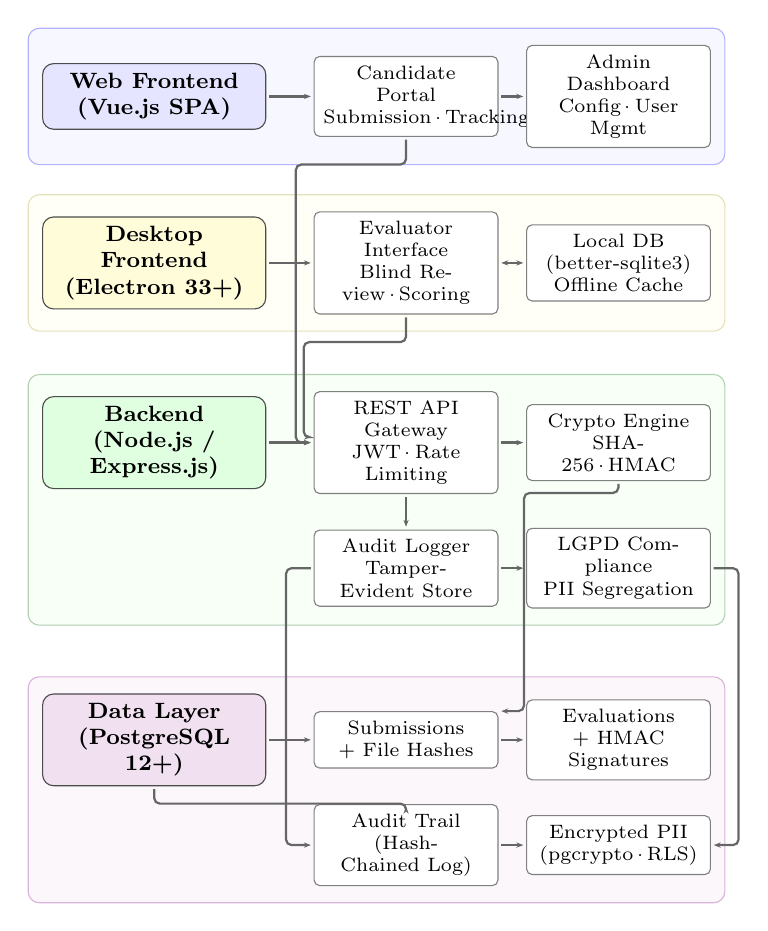
\begin{tikzpicture}[
  node distance=0.45cm and 0.35cm,
  every node/.style={font=\footnotesize},
  layer/.style={rectangle, rounded corners=4pt, draw=black!70, fill=#1,
    minimum height=0.6cm, text width=2.6cm, align=center, font=\footnotesize\bfseries},
  comp/.style={rectangle, rounded corners=2pt, draw=black!50, fill=white,
    minimum height=0.65cm, text width=2.1cm, align=center, font=\scriptsize},
  arr/.style={-{Stealth[length=2.5pt]}, thick, black!60, rounded corners=2pt, shorten <=1pt, shorten >=1pt},
  dblarr/.style={{Stealth[length=2.5pt]}-{Stealth[length=2.5pt]}, thick, black!60, rounded corners=2pt, shorten <=1pt, shorten >=1pt},
  layerlabel/.style={font=\scriptsize\itshape, text=black!55}
]

% ---- WEB FRONTEND ----
\node[layer=blue!10] (web) {Web Frontend\\(Vue.js SPA)};
\node[comp, right=0.6cm of web] (cand) {Candidate Portal\\Submission\,\textperiodcentered\,Tracking};
\node[comp, right=of cand] (admin) {Admin Dashboard\\Config\,\textperiodcentered\,User Mgmt};
\draw[arr] (web) -- (cand);
\draw[arr] (cand) -- (admin);

% ---- DESKTOP FRONTEND ----
\node[layer=yellow!15, below=1.1cm of web] (desk) {Desktop Frontend\\(Electron 33+)};
\node[comp, right=0.6cm of desk] (eval) {Evaluator Interface\\Blind Review\,\textperiodcentered\,Scoring};
\node[comp, right=of eval] (ldb) {Local DB\\(better-sqlite3)\\Offline Cache};
\draw[arr] (desk) -- (eval);
\draw[dblarr] (eval) -- (ldb);

% ---- BACKEND ----
\node[layer=green!12, below=1.1cm of desk] (back) {Backend\\(Node.js / Express.js)};
\node[comp, right=0.6cm of back] (api) {REST API Gateway\\JWT\,\textperiodcentered\,Rate Limiting};
\node[comp, right=of api] (crypto) {Crypto Engine\\SHA-256\,\textperiodcentered\,HMAC};
% segunda linha backend
\node[comp, below=0.45cm of api] (audit) {Audit Logger\\Tamper-Evident Store};
\node[comp, right=of audit] (lgpd) {LGPD Compliance\\PII Segregation};
\draw[arr] (back) -- (api);
\draw[arr] (api) -- (crypto);
\draw[arr] (api.south) -- ++(0,-0.22) -| (audit.north);
\draw[arr] (audit) -- (lgpd);

% ---- DATA LAYER ----
\node[layer=violet!12, below=1.1cm of back |- audit.south] (data) {Data Layer\\(PostgreSQL 12+)};
\node[comp, right=0.6cm of data] (sub) {Submissions\\+ File Hashes};
\node[comp, right=of sub] (evdb) {Evaluations\\+ HMAC Signatures};
\node[comp, below=0.45cm of sub] (atdb) {Audit Trail\\(Hash-Chained Log)};
\node[comp, right=of atdb] (pii) {Encrypted PII\\(pgcrypto\,\textperiodcentered\,RLS)};
\draw[arr] (data) -- (sub);
\draw[arr] (sub) -- (evdb);
\draw[arr] (data.south) -- ++(0,-0.22) -| (atdb.north);
\draw[arr] (atdb) -- (pii);

% ---- INTER-LAYER CONNECTIONS ----
% Left corridor (x~1.55): between layer labels and component boxes
\draw[arr] (cand.south) -- ++(0,-0.35) -- ++(-1.40,0) |- (api.west);
\draw[arr] (eval.south) -- ++(0,-0.35) -- ++(-1.30,0) |- ([yshift=2pt]api.west);
% Mid corridor (x~4.20): between col-2 east and col-3 west
\draw[arr] (crypto.south) -- ++(0,-0.15) -- ++(-1.20,0) |- (sub.north east);
% Audit→Trail: left corridor (avoids sub)
\draw[arr] (audit.west) -- ++(-0.35,0) |- (atdb.west);
% LGPD→PII: right exterior (avoids evdb)
\draw[arr] (lgpd.east) -- ++(0.35,0) |- (pii.east);

% ---- BACKGROUNDS ----
\begin{scope}[on background layer]
  \node[draw=blue!30, rounded corners=4pt, fill=blue!3,
    fit=(web)(cand)(admin), inner xsep=5pt, inner ysep=6pt] {};
  \node[draw=yellow!60!black!30, rounded corners=4pt, fill=yellow!3,
    fit=(desk)(eval)(ldb), inner xsep=5pt, inner ysep=6pt] {};
  \node[draw=green!40!black!30, rounded corners=4pt, fill=green!3,
    fit=(back)(api)(crypto)(audit)(lgpd), inner xsep=5pt, inner ysep=6pt] {};
  \node[draw=violet!30, rounded corners=4pt, fill=violet!3,
    fit=(data)(sub)(evdb)(atdb)(pii), inner xsep=5pt, inner ysep=6pt] {};
\end{scope}
\end{tikzpicture}%
}% end resizebox
\caption{System architecture of avalia+Tec showing the dual-frontend (web portal and desktop application), backend services with cryptographic and compliance modules, and the PostgreSQL data layer with hash-chained audit trail.}
\label{fig:architecture}
\end{figure}

\subsection{Software Functionalities}

The security architecture is grounded in document integrity verification via SHA-256 hashing \citep{NIST2012}, which enables verification of the exact binary correspondence between the evaluated file and the original submission. Simultaneously, the tamper-evident audit log consolidates every state transition (including submission, assignment, evaluation, and decision) in a cryptographically chained ledger. Each entry incorporates the hash of the previous entry, forming a chain: $H_n = \text{SHA-256}(\text{event}_n \| H_{n-1})$. This sequential chaining renders retroactive modification of any individual entry \emph{detectable}, as it would invalidate all subsequent hashes \citep{Bellare1997}. To strengthen tamper-evidence beyond internal database controls, the platform implements external hash anchoring via RFC~3161-compliant Timestamp Authorities (TSA). Upon each submission, the computed SHA-256 digest is submitted to an independent TSA (default: FreeTSA.org), which returns a signed TimeStampResp (TSR) token containing the hash, a trusted timestamp, and the TSA's digital signature. This TSR is stored alongside the submission record. Even a server administrator with root-level database access cannot forge a valid TSR, as doing so would require the TSA's private signing key \citep{RFC3161}.

The submission pipeline operates as follows: candidates access the web portal, authenticate, and complete a dynamic form configured per campaign (Fig.~\ref{fig:webportal}). Upon submission, the server computes a SHA-256 hash of each upload, stores the file on encrypted storage, and issues a unique protocol ID and a verification hash printed on the candidate's receipt. The evaluation workflow segregates evaluator roles by institutional function, with configurable visibility rules that hide candidate names to reduce bias.

\begin{figure}[H]
\centering
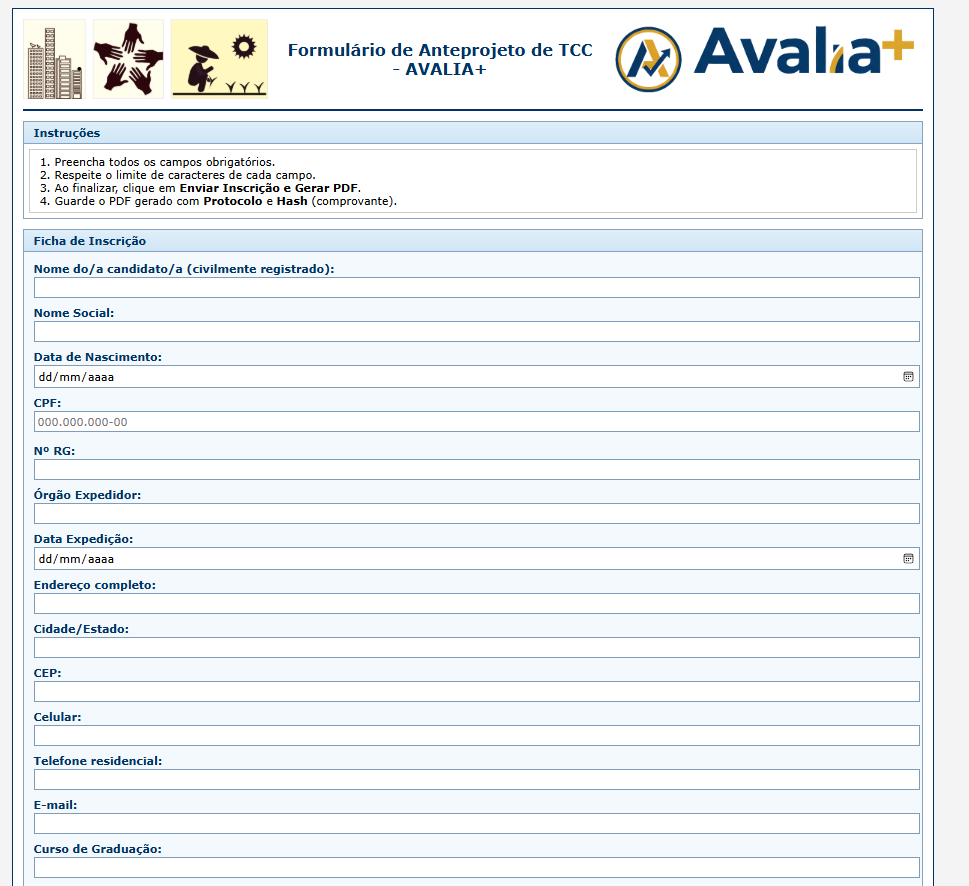
\includegraphics[width=0.92\textwidth]{fig-web-portal.png}
\caption{Web portal interface showing the candidate submission form with structured sections, field-level validation, and real-time character count enforcement.}
\label{fig:webportal}
\end{figure}

Evaluators authenticate to the desktop application (Fig.~\ref{fig:blindreview}), which synchronizes submissions and supports offline scoring. Scorecards are authenticated via HMAC-SHA256 \citep{Bellare1997} before transmission, providing cryptographic attestation of evaluator identity and score integrity.

\begin{figure}[H]
\centering
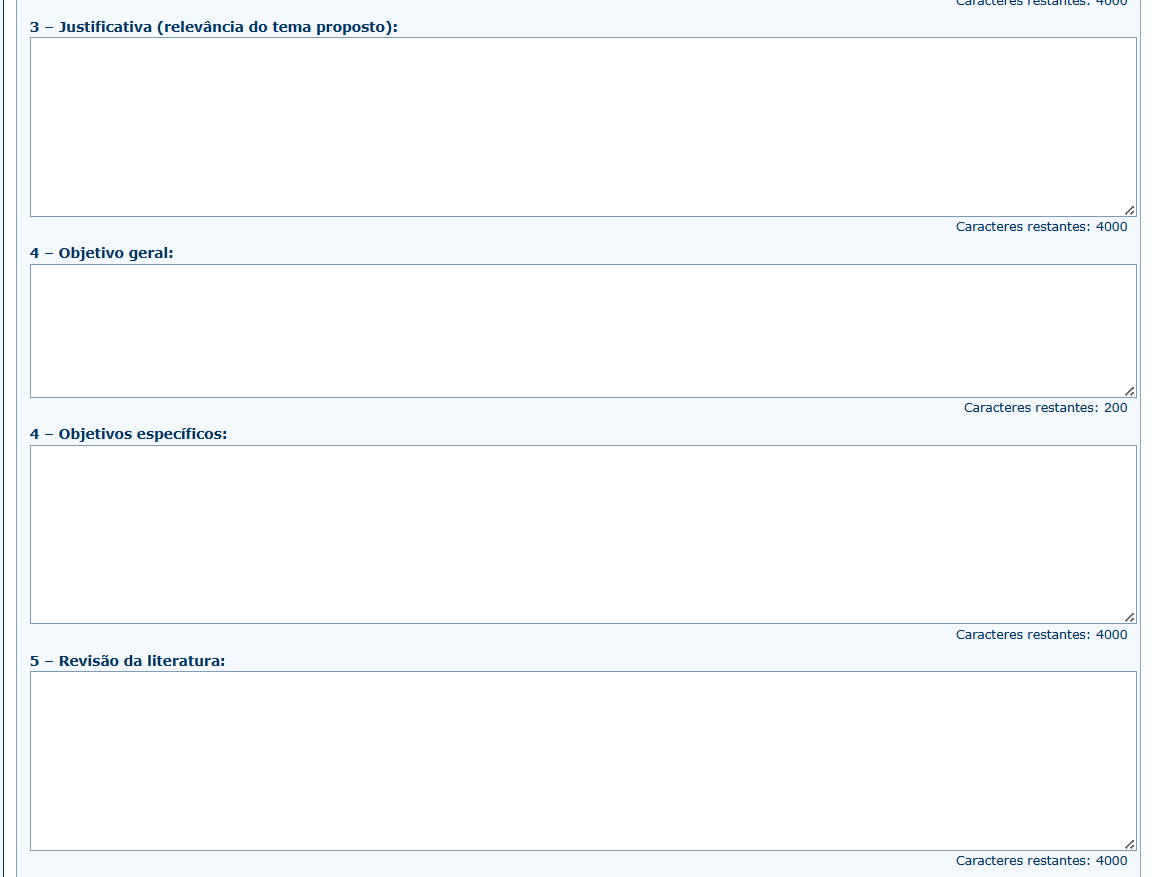
\includegraphics[width=0.92\textwidth]{fig-desktop-blindreview.png}
\caption{Desktop application (Electron) displaying the evaluator's blind-review interface. Personally identifiable candidate information is suppressed to enforce impartial assessment.}
\label{fig:blindreview}
\end{figure}

Consolidation is automated, and once all evaluations are recorded the server computes weighted aggregates and generates rank-ordered lists with full derivation trail in the audit log. The complete data flow follows a linear pipeline in which each candidate submission is first hashed (SHA-256) and anchored via TSA, then assigned to evaluators for blind scoring with HMAC authentication. Server-side validation and audit logging precede automated consolidation, which produces PII-redacted result publication. Every state transition is appended to the hash-chained audit trail.

\textbf{LGPD-aware design.} The platform implements technical controls supporting LGPD compliance through data segregation: evaluator records and PII are stored in separate database tables with role-based access control enforced at the PostgreSQL row-level security (RLS) layer. Encrypted-at-rest protection via pgcrypto secures sensitive fields (CPF, RG, contact information), and automated redaction strips non-essential PII from public result exports \citep{McGraw2006}. Table~\ref{tab:lgpdmapping} maps specific LGPD provisions to the corresponding technical mechanisms implemented in avalia+Tec. Although primarily designed for LGPD (Brazil), the underlying technical controls (purpose-limited data collection, encryption at rest and in transit, role-based access, automated PII redaction, and auditable processing logs) align with core principles of the EU General Data Protection Regulation (GDPR), particularly Articles~5 (data minimization, integrity), 25 (data protection by design), and 32 (security of processing) \citep{GDPR2016}. Institutions operating under GDPR or similar frameworks can therefore adopt the platform with jurisdiction-specific policy adaptations. Full compliance requires organizational, legal, and technical measures; this platform provides the technical layer, while institutional policy, Data Protection Impact Assessment (DPIA), and legal review remain the responsibility of the deploying organization.

\begin{table}[H]
\centering
\footnotesize
\begin{tabular}{|l|p{3.5cm}|p{5.5cm}|}
\hline
\textbf{LGPD Art.} & \textbf{Requirement} & \textbf{Technical Control in avalia+Tec} \\
\hline
Art. 6, I--II & Purpose limitation \& adequacy & Data fields scoped to selection process; no secondary processing \\
\hline
Art. 6, V & Data quality & SHA-256 integrity verification prevents silent corruption \\
\hline
Art. 6, VII--VIII & Security \& prevention & Encrypted storage (pgcrypto), TLS in transit, rate limiting, attack pattern detection \\
\hline
Art. 6, X & Accountability & Hash-chained audit trail with external TSA anchoring (RFC 3161) \\
\hline
Art. 46 & Security measures & RBAC, RLS, helmet.js headers, JWT authentication, IP allowlisting for admin routes \\
\hline
Art. 48 & Incident notification & Structured security logging (Winston) with rotation; security event taxonomy \\
\hline
Art. 18 & Data subject rights & Automated PII redaction in public exports; data accessible via protocol ID \\
\hline
\end{tabular}
\caption{Mapping of LGPD provisions to technical controls implemented in avalia+Tec. Full compliance additionally requires institutional policies, DPIA, and legal assessment.}
\label{tab:lgpdmapping}
\end{table}

%% ============================================================
\section{Illustrative Examples}
%% ============================================================

Consider a scholarship selection campaign at a public university. The institution creates a campaign via the administrative portal, configuring evaluation criteria with weighted rubrics (e.g., technical merit 0.4, social vulnerability 0.3, leadership 0.3). Candidates register, upload required documents, and submit via the web portal. The server computes SHA-256 hashes of all uploads and issues a receipt containing the submission timestamp, a unique protocol ID (e.g., SCH-2026-0447), and the hexadecimal verification hash. Listing~\ref{lst:hashcompute} presents the server-side implementation of the SHA-256 document hashing mechanism.

\begin{lstlisting}[language=JavaScript, caption={Server-side SHA-256 hash computation upon document upload. The hash is stored in the database and returned to the candidate as a verification receipt.}, label=lst:hashcompute]
const crypto = require('crypto');
const fs = require('fs');

async function computeDocumentHash(filePath) {
  const hash = crypto.createHash('sha256');
  const stream = fs.createReadStream(filePath);
  for await (const chunk of stream) {
    hash.update(chunk);
  }
  return hash.digest('hex');
}

// Submission upload endpoint
app.post('/api/submissions/:id/upload',
  authenticate, async (req, res) => {
  const sha256 = await computeDocumentHash(
    req.file.path);
  await db.query(
    `INSERT INTO document_hashes
     (submission_id, file_hash, created_at)
     VALUES ($1, $2, NOW())`,
    [req.params.id, sha256]
  );
  res.json({ protocolId: generateProtocolId(),
             hash: sha256 });
});
\end{lstlisting}

Seven faculty evaluators are provisioned and assigned to criteria sections. Each evaluator logs into the desktop application and sees only anonymized content (candidate names hidden). Scores are entered on a structured rubric, and the desktop app authenticates each scorecard via HMAC-SHA256 before uploading. The server validates message authentication codes, logs evaluation events, and prevents cross-evaluator score visibility. Listing~\ref{lst:verify} shows the integrity verification endpoint available to auditors and candidates.

\begin{lstlisting}[language=JavaScript, caption={Document integrity verification endpoint. Compares the stored hash against a freshly computed hash to detect post-submission modification.}, label=lst:verify]
app.get('/api/verify/:protocolId',
  authenticate, async (req, res) => {
  const record = await db.query(
    `SELECT file_path, file_hash
     FROM document_hashes
     WHERE protocol_id = $1`,
    [req.params.protocolId]
  );
  const currentHash = await computeDocumentHash(
    record.rows[0].file_path);
  const verified =
    currentHash === record.rows[0].file_hash;
  res.json({
    protocolId: req.params.protocolId,
    originalHash: record.rows[0].file_hash,
    currentHash: currentHash,
    integrityVerified: verified
  });
});
\end{lstlisting}

Table~\ref{tab:auditsample} presents a representative excerpt of the hash-chained audit trail generated during the UEFS deployment.

\begin{table}[H]
\centering
\footnotesize
\begin{tabular}{|c|l|l|l|l|}
\hline
\textbf{\#} & \textbf{Timestamp} & \textbf{Actor} & \textbf{Action} & \textbf{$H_n$ (truncated)} \\
\hline
1 & 2025-03-15 09:12:34 & system & Submission received & \texttt{a3f7c2...8d1e} \\
\hline
2 & 2025-03-15 09:12:35 & system & SHA-256 computed & \texttt{7b2e4f...93a2} \\
\hline
3 & 2025-03-18 14:22:11 & eval\_03 & Score recorded (4.2) & \texttt{d91c8a...f7b3} \\
\hline
4 & 2025-03-18 14:22:12 & system & HMAC validated & \texttt{e4a6b1...2c7d} \\
\hline
5 & 2025-04-02 10:05:47 & system & Consolidation finalized & \texttt{f82d3e...a104} \\
\hline
6 & 2025-04-02 10:05:48 & system & Results published & \texttt{1c9f7a...b5e8} \\
\hline
\end{tabular}
\caption{Representative excerpt of the hash-chained audit trail from the UEFS deployment. Each hash $H_n$ incorporates the previous entry's hash $H_{n-1}$, ensuring tamper-evidence across the entire chain.}
\label{tab:auditsample}
\end{table}

Each hash-chained entry belongs to one of four workflow phases (submission, blind evaluation, automated consolidation, and dispute resolution) whose cryptographic checkpoints and verification logic are mapped in Fig.~\ref{fig:auditflow}.

%%% ---- FIGURE 4: AUDIT TRAIL FLOWCHART (TikZ) ----
\begin{figure}[H]
\centering
\resizebox{\textwidth}{!}{%
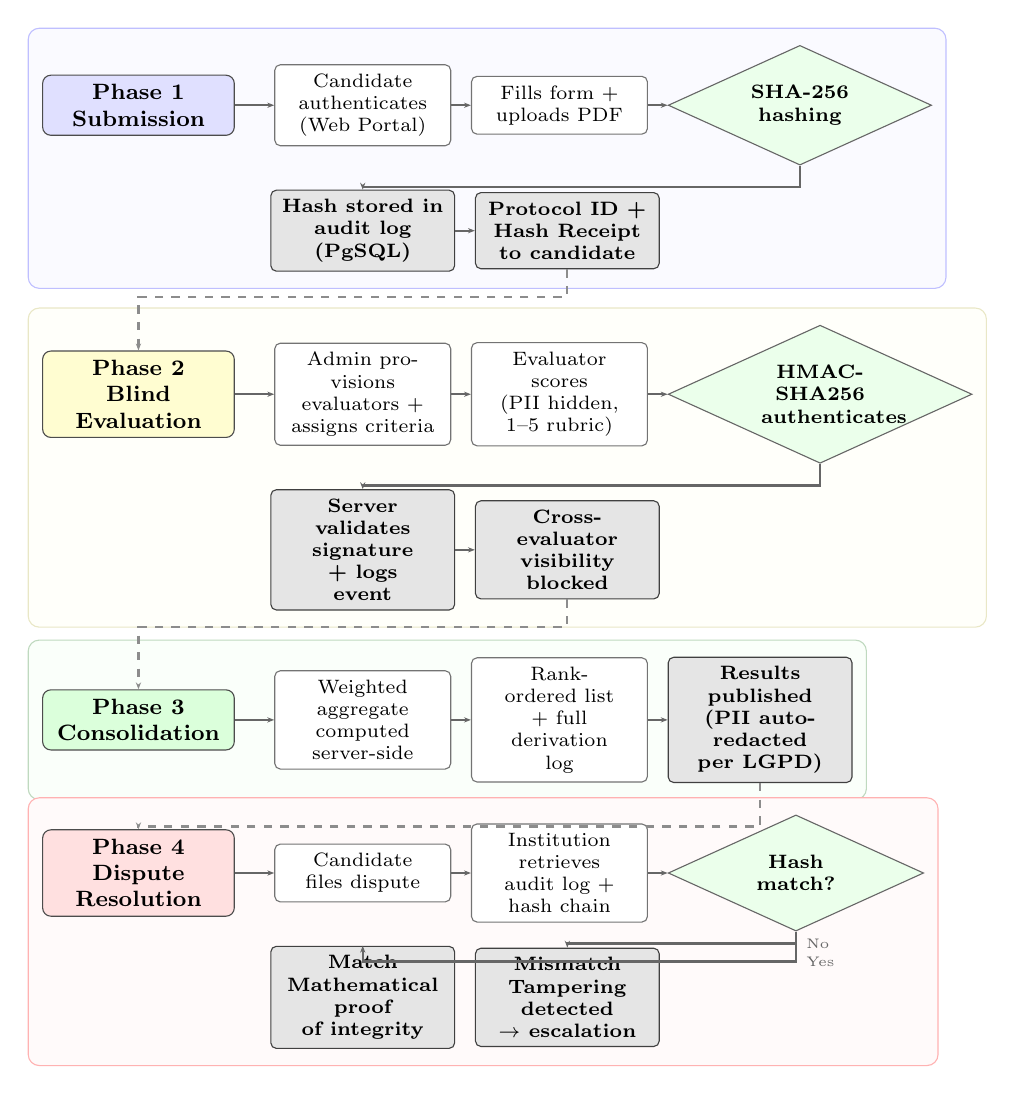
\begin{tikzpicture}[
  node distance=0.4cm and 0.25cm,
  every node/.style={font=\footnotesize},
  phase/.style={rectangle, rounded corners=3pt, draw=black!70, fill=#1,
    minimum height=0.55cm, text width=2.2cm, align=center, font=\footnotesize\bfseries},
  stepbox/.style={rectangle, rounded corners=2pt, draw=black!55, fill=white,
    minimum height=0.65cm, text width=2.0cm, align=center, font=\scriptsize},
  cryptobox/.style={diamond, draw=black!60, fill=green!8, aspect=2.2,
    minimum height=0.5cm, text width=1.5cm, align=center, font=\scriptsize\bfseries},
  output/.style={rectangle, rounded corners=2pt, draw=black!75, fill=black!10,
    minimum height=0.65cm, text width=2.1cm, align=center, font=\scriptsize\bfseries},
  arr/.style={-{Stealth[length=2.5pt]}, thick, black!60},
  dashline/.style={-{Stealth[length=2.5pt]}, thick, black!45, dashed}
]

% ===== PHASE 1: SUBMISSION =====
\node[phase=blue!12] (p1) {Phase 1\\Submission};
\node[stepbox, right=0.5cm of p1] (s1) {Candidate\\authenticates\\(Web Portal)};
\node[stepbox, right=of s1] (s2) {Fills form +\\uploads PDF};
\node[cryptobox, right=of s2] (s3) {SHA-256\\hashing};
\draw[arr] (p1) -- (s1);
\draw[arr] (s1) -- (s2);
\draw[arr] (s2) -- (s3);
% outputs phase 1
\node[output, below=0.55cm of s1] (s4) {Hash stored in\\audit log (PgSQL)};
\node[output, right=of s4] (s5) {Protocol ID +\\Hash Receipt\\to candidate};
\draw[arr] (s3.south) -- ++(0,-0.275) -| (s4.north);
\draw[arr] (s4) -- (s5);

% ===== PHASE 2: BLIND EVALUATION =====
\node[phase=yellow!18, below=1.0cm of p1 |- s4.south] (p2) {Phase 2\\Blind Evaluation};
\node[stepbox, right=0.5cm of p2] (e1) {Admin provisions\\evaluators +\\assigns criteria};
\node[stepbox, right=of e1] (e2) {Evaluator scores\\(PII hidden,\\1--5 rubric)};
\node[cryptobox, right=of e2] (e3) {HMAC-SHA256\\authenticates};
\draw[arr] (p2) -- (e1);
\draw[arr] (e1) -- (e2);
\draw[arr] (e2) -- (e3);
% outputs phase 2
\node[output, below=0.55cm of e1] (e4) {Server validates\\signature + logs\\event};
\node[output, right=of e4] (e5) {Cross-evaluator\\visibility blocked};
\draw[arr] (e3.south) -- ++(0,-0.275) -| (e4.north);
\draw[arr] (e4) -- (e5);

% ===== PHASE 3: CONSOLIDATION =====
\node[phase=green!14, below=1.0cm of p2 |- e4.south] (p3) {Phase 3\\Consolidation};
\node[stepbox, right=0.5cm of p3] (c1) {Weighted aggregate\\computed\\server-side};
\node[stepbox, right=of c1] (c2) {Rank-ordered list\\+ full derivation\\log};
\node[output, right=of c2] (c3) {Results published\\(PII auto-redacted\\per LGPD)};
\draw[arr] (p3) -- (c1);
\draw[arr] (c1) -- (c2);
\draw[arr] (c2) -- (c3);

% ===== PHASE 4: DISPUTE RESOLUTION =====
\node[phase=red!12, below=1.0cm of p3] (p4) {Phase 4\\Dispute Resolution};
\node[stepbox, right=0.5cm of p4] (d1) {Candidate\\files dispute};
\node[stepbox, right=of d1] (d2) {Institution retrieves\\audit log +\\hash chain};
\node[cryptobox, right=of d2] (d3) {Hash\\match?};
\draw[arr] (p4) -- (d1);
\draw[arr] (d1) -- (d2);
\draw[arr] (d2) -- (d3);
% outputs phase 4 — decision branches
\node[output, below=0.55cm of d1] (d4) {\textbf{Match}\\Mathematical proof\\of integrity};
\node[output, right=of d4] (d5) {\textbf{Mismatch}\\Tampering detected\\$\rightarrow$ escalation};
\draw[arr] (d3.south) -- ++(0,-0.38) node[right, font=\tiny]{Yes} -| (d4.north);
\draw[arr] (d3.south) -- ++(0,-0.15) node[right, font=\tiny]{No} -| (d5.north);

% ===== INTER-PHASE CONNECTORS =====
\draw[dashline] (s5.south) -- ++(0,-0.35) -| (p2.north);
\draw[dashline] (e5.south) -- ++(0,-0.35) -| (p3.north);
\draw[dashline] (c3.south) -- ++(0,-0.55) -| (p4.north);

% ===== BACKGROUNDS =====
\begin{scope}[on background layer]
  \node[draw=blue!25, rounded corners=4pt, fill=blue!2,
    fit=(p1)(s1)(s2)(s3)(s4)(s5), inner xsep=5pt, inner ysep=6pt] {};
  \node[draw=yellow!60!black!25, rounded corners=4pt, fill=yellow!2,
    fit=(p2)(e1)(e2)(e3)(e4)(e5), inner xsep=5pt, inner ysep=6pt] {};
  \node[draw=green!40!black!25, rounded corners=4pt, fill=green!2,
    fit=(p3)(c1)(c2)(c3), inner xsep=5pt, inner ysep=6pt] {};
  \node[draw=red!30, rounded corners=4pt, fill=red!2,
    fit=(p4)(d1)(d2)(d3)(d4)(d5), inner xsep=5pt, inner ysep=6pt] {};
\end{scope}
\end{tikzpicture}%
}% end resizebox
\caption{End-to-end audit trail flowchart showing cryptographic operations (SHA-256 hashing, HMAC-SHA256 authentication) and verification checkpoints across four phases: document submission, blind evaluation, automated consolidation, and dispute resolution with hash-based integrity verification.}
\label{fig:auditflow}
\end{figure}

After all evaluations are complete, the system computes weighted averages (e.g., Application \#23 receives $(4 \times 0.4) + (5 \times 0.3) + (2 \times 0.3) = 3.7$), ranks submissions, and publishes results with automatic PII redaction (Fig.~\ref{fig:consolidation}). If a candidate files a dispute, the institution retrieves the cryptographic audit log: the SHA-256 hash provides strong evidence that the document has not been altered, HMAC authentication codes attest that evaluator scores have not been modified, and the complete derivation log shows exactly which scores were aggregated, by whom, and when. The candidate's original submission receipt, containing the protocol ID and SHA-256 verification hash (Fig.~\ref{fig:protocolhash}), provides independent evidence of document integrity. In the observed deployment, this evidence contributed to rapid dispute resolution without escalation.

\textbf{Threat model.} The security architecture addresses three adversary classes:

\begin{enumerate}
  \item \textbf{External adversary} (unauthenticated attacker): Mitigated by TLS encryption, rate limiting, input sanitization, attack pattern detection (SQL injection, XSS, path traversal), and JWT-based authentication. Security headers (helmet.js) prevent clickjacking and content-type sniffing.
  \item \textbf{Insider, non-privileged user} (authenticated candidate or evaluator): Mitigated by RBAC, PostgreSQL row-level security (RLS), cross-evaluator visibility blocking, HMAC-SHA256 scorecard authentication, and the hash-chained audit trail that makes any unauthorized modification detectable.
  \item \textbf{Insider, privileged administrator} (root-level database access): This is the most challenging adversary. A malicious administrator could, in principle, modify records and rewrite the internal hash chain consistently. To mitigate this threat, avalia+Tec implements external hash anchoring via RFC~3161-compliant Timestamp Authorities (TSA). Each submission hash is independently timestamped by an external TSA (default: FreeTSA.org), producing a signed TimeStampResp token that the administrator cannot forge without the TSA's private key. This provides \emph{independently verifiable} evidence of document existence and integrity at a specific point in time.
\end{enumerate}

\textbf{Residual limitations.} The RFC~3161 anchoring mitigates but does not fully eliminate the trusted-administrator threat: if the administrator suppresses the TSR storage \emph{before} the timestamp is requested, no external anchor exists for that record. Future work will explore continuous external anchoring (e.g., periodic checkpoint publication to a public blockchain) and multi-party key management to further reduce this residual risk. No formal penetration testing or external security audit has been conducted to date; this represents planned future work. The current implementation has been assessed against the OWASP Top~10 checklist \citep{Owasp2023}, and \texttt{npm audit} reports zero known high-severity vulnerabilities in production dependencies.

\begin{figure}[H]
\centering
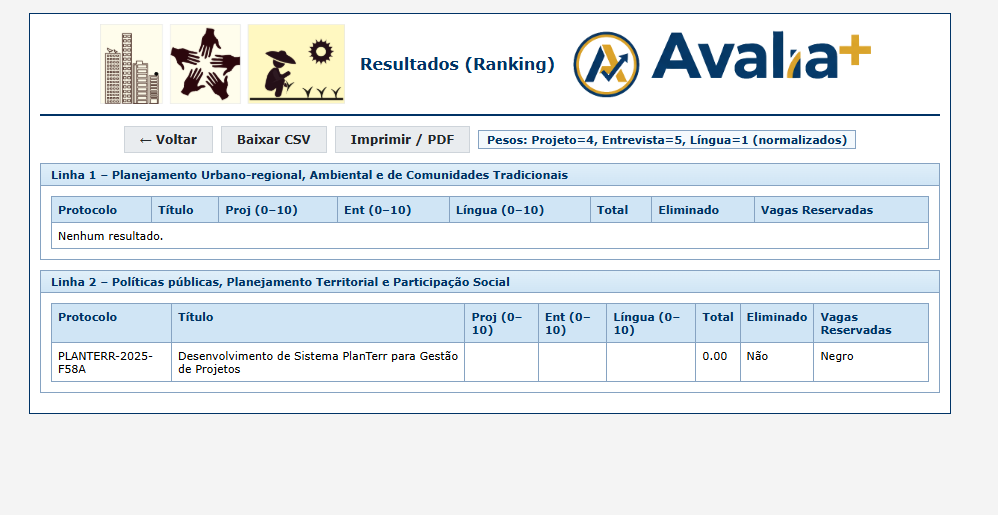
\includegraphics[width=0.92\textwidth]{fig-consolidation.png}
\caption{Consolidation dashboard showing rank-ordered results with weighted aggregate scores, individual evaluator contributions, and export options (CSV, PDF with QR-code verification).}
\label{fig:consolidation}
\end{figure}

\begin{figure}[H]
\centering
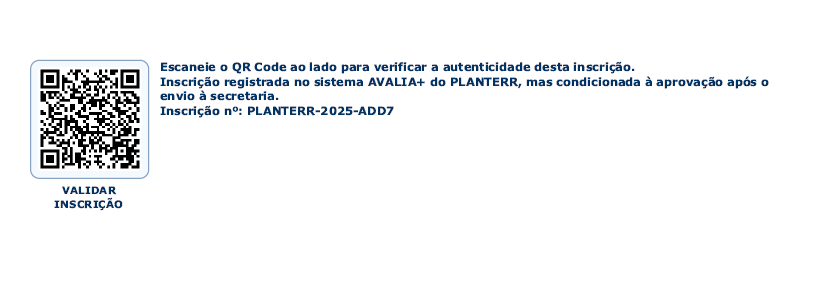
\includegraphics[width=0.75\textwidth]{fig-protocol-hash.png}
\caption{Candidate receipt (PDF) displaying the unique protocol ID, submission timestamp, and SHA-256 hexadecimal hash for independent document integrity verification. The embedded QR code links to the audit trail endpoint.}
\label{fig:protocolhash}
\end{figure}

%% ============================================================
\section{Computational Performance}
%% ============================================================

To characterize the computational overhead introduced by the cryptographic operations, we measured the execution time of core platform operations during the UEFS deployment. The server infrastructure consists of an AWS EC2 t3.medium instance (2 vCPUs, 4~GB RAM) running Ubuntu 22.04~LTS, PostgreSQL~15.4, and Node.js~18.19. Network connectivity between the desktop client and the server was measured over the institutional 100~Mbps Ethernet connection. Each operation was executed 30 times, and summary statistics are reported in Table~\ref{tab:performance}.

\begin{table}[H]
\centering
\footnotesize
\begin{tabular}{|l|c|c|}
\hline
\textbf{Operation} & \textbf{Mean (SD)} & \textbf{Median [$Q_1$, $Q_3$]} \\
\hline
SHA-256 hash (1~MB PDF) & 12.4~ms (2.1) & 11.9~ms [11.2, 13.1] \\
\hline
SHA-256 hash (5~MB PDF) & 47.3~ms (5.8) & 46.1~ms [43.2, 50.7] \\
\hline
HMAC-SHA256 scorecard auth. & 1.8~ms (0.3) & 1.7~ms [1.6, 1.9] \\
\hline
Audit trail append & 3.2~ms (0.9) & 3.0~ms [2.7, 3.5] \\
\hline
Desktop $\leftrightarrow$ server sync (60 subs.) & 4.25~s (0.38) & 4.18~s [4.02, 4.41] \\
\hline
Consolidation (60 $\times$ 6 evals) & 0.89~s (0.12) & 0.87~s [0.81, 0.94] \\
\hline
\end{tabular}
\caption{Computational time associated with core avalia+Tec operations. Measurements were collected over 30 executions on an AWS EC2 t3.medium instance (2~vCPUs, 4~GB RAM, Ubuntu 22.04 LTS).}
\label{tab:performance}
\end{table}

From Table~\ref{tab:performance}, the cryptographic operations (SHA-256 hashing and HMAC-SHA256 authentication) impose negligible overhead relative to user-perceived latency: even for a 5~MB PDF document, hash computation completes in under 50~ms. The most time-intensive operation is the desktop-to-server synchronization, which transfers all submission metadata and files; at 4.25~s for 60 submissions, this remains well within acceptable limits for evaluator session initialization. The automated consolidation of 360 individual evaluations (60 submissions $\times$ 6 evaluators) completes in under one second, eliminating the manual consolidation step that previously required approximately 4~hours of administrative staff time per campaign cycle.

\subsection{Load Testing}

To assess scalability beyond the initial deployment scale, we conducted stress tests using autocannon (Node.js HTTP benchmarking tool) with the server running in JSON storage mode. Table~\ref{tab:loadtest} reports results for two concurrency levels.

\begin{table}[H]
\centering
\footnotesize
\begin{tabular}{|l|c|c|c|c|c|}
\hline
\textbf{Scenario} & \textbf{Conc.} & \textbf{Req/s} & \textbf{$p_{50}$ (ms)} & \textbf{$p_{97.5}$ (ms)} & \textbf{$p_{99}$ (ms)} \\
\hline
GET / (landing) & 100 & 1{,}753 & 52 & 98 & 113 \\
 & 500 & 1{,}717 & 259 & 563 & 677 \\
\hline
GET /api/verify & 100 & 1{,}560 & 62 & 143 & 248 \\
 & 500 & 2{,}061 & 283 & 427 & 501 \\
\hline
POST /api/inscricao & 100 & 1{,}338 & 68 & 133 & 289 \\
 & 500 & 1{,}599 & 487 & 6{,}241 & 8{,}153 \\
\hline
\end{tabular}
\caption{Load test results (30~seconds per scenario, autocannon). Conc.\ = concurrent connections. Raw results are available in the replication package (\texttt{load\_test\_results.json}).}
\label{tab:loadtest}
\end{table}

Read-heavy operations (landing page, integrity verification) sustain over 1{,}500 req/s at both concurrency levels. Write-heavy operations (submission creation with SHA-256 hashing and database insertion) maintain high throughput at 100 connections but exhibit significant tail latency at 500 connections ($p_{99} = 8{,}153$~ms), indicating the single-threaded event loop saturation point. For the target deployment scale (tens to hundreds of concurrent users during submission windows), the current single-instance architecture provides adequate performance. Horizontal scaling via load balancing and PostgreSQL read replicas represents a straightforward architectural extension for larger deployments.

%% ============================================================
\section{Impact}
%% ============================================================

avalia+Tec has been operationally deployed at Universidade Estadual de Feira de Santana (UEFS). Over a 12-month period (calendar year 2025), the platform processed 60 submissions for professional master's degree admissions. Telemetry collected across four evaluation sessions ($n = 6$ evaluators, 65 evaluation events) yielded the following preliminary observations.

In terms of process efficiency, the average review-to-decision cycle time decreased from 31 calendar days (SD = 4.2, $n = 4$ historical campaigns) to 11 days (SD = 2.8, $n = 4$ sessions)---a 65\% reduction (95\% CI: [55\%, 73\%]; Mann--Whitney $U = 0$, $p = 0.029$, two-tailed; rank-biserial $r = 1.0$). This improvement is attributable to the elimination of manual consolidation and spreadsheet version control, translating to an estimated 15 staff-hours saved per campaign. Given the small number of campaign cycles ($n = 4$ per condition), these results should be interpreted as preliminary effect-size estimates rather than definitive causal conclusions. The pre--post observational design without randomization cannot fully control for confounding factors such as changes in administrative staff composition or learning effects.

Regarding formal disputes, in contrast to the historical complaint rate of approximately 4.8\% observed under previous processes at UEFS (14 complaints across 292 submissions over 3 years), no formal complaints were registered during the observation period ($0/60$ submissions). A one-tailed Fisher's exact test comparing 0/60 vs.\ 14/292 yields $p = 0.069$, which does not reach conventional significance at $\alpha = 0.05$. The small sample size precludes definitive statistical conclusions. The availability of cryptographic audit logs may have contributed to discouraging disputes by providing verifiable evidence of procedural regularity \citep{Hood2007}.

As for evaluator experience, the average evaluation time per submission was $T = 8.3 \pm 2.1$~min (mean $\pm$ SD, $n = 6$ evaluators, 65 evaluations), compared to $T' = 15.2 \pm 4.7$~min under previous workflows (retrospective administrative survey, same $n = 6$ evaluators), representing a 45.4\% reduction (95\% CI: [26\%, 59\%]; Mann--Whitney $U = 2$, $p = 0.009$, two-tailed; Cohen's $d = 1.88$, large effect). These baseline measurements derive from retrospective self-reported data and are therefore subject to recall bias; evaluators may overestimate prior time expenditure. Additionally, evaluator time measurements under the new system may be influenced by the Hawthorne effect, as evaluators were aware of the system's monitoring capabilities. Technical support requests declined approximately 58\% due to the improved user autonomy afforded by the system.

Finally, concerning maintenance and availability, the software is maintained as an open-source project (MIT License) on GitHub \citep{AvaliaMoreGitHub2026,AvaliaMoreDesktop2026}, with continuous integration via GitHub Actions, a public issue tracker, semantic versioning, and bilingual documentation (Portuguese and English) \citep{Sommerville2016}. The platform has been formally registered as a computer program with the Brazilian National Institute of Industrial Property (INPI) under Process No.\ 512026000776-3, securing intellectual property protection without compromising open-source availability.

%% ============================================================
\section{Limitations}
%% ============================================================

\textbf{Study design.} This is a single-institution, pre--post observational study without a randomized control group. The deployment involved a relatively small sample ($n = 60$ submissions, $n = 6$ evaluators), which limits statistical power and external generalizability. While we report Mann--Whitney $U$ tests, confidence intervals, and effect sizes (Section~5), these should be interpreted as preliminary evidence. Multi-institutional deployments with larger samples and, ideally, randomized or quasi-experimental designs are needed to confirm the observed effects.

\textbf{Baseline data quality.} Comparisons with previous workflows rely on retrospective self-reported data from administrative surveys and are subject to recall bias. Evaluators may overestimate prior time expenditure, inflating the apparent efficiency gain. No objective time-tracking data exists for the pre-deployment period.

\textbf{Security.} As discussed in Section~3, the threat model addresses privileged insiders via RFC~3161 external timestamp anchoring. However, no formal penetration testing or external security audit has been conducted. Key management practices (JWT secrets, HMAC keys stored as environment variables, not hardcoded) follow standard recommendations but have not been independently verified. The implementation has been checked against the OWASP Top~10 \citep{Owasp2023} and \texttt{npm audit} reports zero high-severity vulnerabilities, but these do not constitute a comprehensive security assessment.

\textbf{LGPD compliance.} The platform provides technical controls supporting LGPD compliance (Table~\ref{tab:lgpdmapping}), but full compliance requires organizational policies, a formal Data Protection Impact Assessment (DPIA), and legal review by each deploying institution. No formal DPIA has been conducted for the current deployment.

\textbf{Reproducibility.} Anonymized deployment metrics and analysis scripts are available at \url{https://doi.org/10.5281/zenodo.18868994} to support reproducibility.

%% ============================================================
\section{Conclusions}
%% ============================================================

avalia+Tec addresses an underserved need in institutional informatics: the transparent, procedurally accountable, and LGPD-aware governance of competitive selection processes. Preliminary deployment results from a single-institution observational study suggest that the systematic integration of well-established cryptographic techniques into a unified, open-source workflow is associated with meaningful reductions in administrative cycle time (65\%, 95\% CI: [55\%, 73\%]) and evaluator workload (45.4\%, 95\% CI: [26\%, 59\%]), while providing tamper-evident cryptographic evidence of document authenticity and procedural fairness. No formal disputes were observed during the monitoring period, though the sample size precludes definitive conclusions. The combination of hash-based integrity verification with external RFC~3161 timestamp anchoring, HMAC-authenticated scorecards, tamper-evident hash-chained audit trails, and role-based data segregation constitutes a reproducible integration engineering blueprint applicable to institutions that manage competitive selection under legal accountability requirements. The scientific contribution resides in this systematic integration rather than in the underlying cryptographic primitives. The platform is freely available under the MIT License and suitable for adoption by universities, funding agencies, and public-sector organizations. Future work will target larger-scale multi-institutional deployments with formal statistical evaluation, including randomized or quasi-experimental designs. Planned technical extensions include API integration with institutional student information systems (e.g., SIGAA, SUAP), continuous external hash anchoring through periodic blockchain checkpoint publication, and formal penetration testing with independent security audits. Identity management may be strengthened through federated authentication via SAML/OAuth~2.0 with institutional identity providers, while long-term audit storage could benefit from tiered archival strategies with cryptographic integrity seals for regulatory retention periods. Additional work will address Data Protection Impact Assessments and the development of fairness auditing modules capable of detecting systematic evaluator biases from the structured data that the platform collects. An independent external security audit is currently budgeted and planned for the next development cycle to complement the existing automated dependency and OWASP-based assessments.

%% ============================================================
\section*{Acknowledgements}
%% ============================================================

The authors acknowledge the contribution of the avalia+ development team and the institutional support of Universidade Estadual de Feira de Santana (UEFS).

%% ============================================================
\section*{CRediT authorship contribution statement}
%% ============================================================

\textbf{Luiz Diego Vidal Santos:} Conceptualization, Methodology, Software, Validation, Formal analysis, Investigation, Data curation, Writing -- original draft, Writing -- review \& editing, Visualization, Project administration. \textbf{Catuxe Varjão de Santana Oliveira:} Conceptualization, Methodology, Validation, Formal analysis, Writing -- review \& editing, Supervision. \textbf{Dulce Paloma Vidal Santos:} Investigation, Validation. \textbf{Tânia Cristina Azevedo:} Resources, Supervision. \textbf{Renisson Neponuceno de Araújo Filho:} Writing -- review \& editing. \textbf{Jémison Mattos dos Santos:} Writing -- review \& editing. \textbf{Milton Marques Fernandes:} Writing -- review \& editing. \textbf{Francisco Sandro Rodrigues Holanda:} Writing -- review \& editing.

%% ============================================================
\section*{Declaration of competing interest}
%% ============================================================

The authors declare that they have no known competing financial interests or personal relationships that could have appeared to influence the work reported in this paper.

%% ============================================================
\section*{Data availability}
%% ============================================================

The source code and documentation are publicly available at \url{https://github.com/ldvsantos/avalia_mais} (server and web portal) and \url{https://github.com/ldvsantos/avalia_mais_desktop} (desktop application). The software is registered with INPI (Brazil) under Process No. 512026000776-3. Anonymized deployment metrics, statistical analysis scripts (Python), and the load testing framework are available in the replication package at \url{https://doi.org/10.5281/zenodo.18868994}.

\appendix

\section{Deployment and Environment Setup}
\label{app:deployment}

This appendix provides the essential commands for deploying avalia+Tec in a production environment. The setup assumes a Linux server (Ubuntu 22.04~LTS) with PostgreSQL~12+ and Node.js~18+ installed.

\begin{lstlisting}[language=sh, caption={Server-side deployment of the avalia+Tec backend and web portal. The script clones the repository, installs dependencies, configures the database, and starts the application.}, label=lst:deploy]
#!/bin/bash
# Clone repository and install dependencies
git clone https://github.com/ldvsantos/avalia_mais.git
cd avalia_mais
npm install --production

# Configure environment variables
cp .env.example .env
# Edit .env with database credentials and JWT secret
# DB_HOST=localhost  DB_PORT=5432
# DB_NAME=avalia_db  DB_USER=avalia_admin
# JWT_SECRET=$(openssl rand -hex 32)

# Initialize PostgreSQL database with pgcrypto
sudo -u postgres psql -c \
  "CREATE DATABASE avalia_db;"
sudo -u postgres psql -d avalia_db -c \
  "CREATE EXTENSION IF NOT EXISTS pgcrypto;"
npm run db:migrate
npm run db:seed    # optional demo data

# Start application (production mode)
NODE_ENV=production npm start
# Server listens on port 3000 by default
\end{lstlisting}

\begin{lstlisting}[language=sh, caption={Building the Electron desktop application for evaluators. Produces platform-specific installers for Windows, macOS, and Linux.}, label=lst:desktopbuild]
#!/bin/bash
# Clone desktop repository
git clone \
  https://github.com/ldvsantos/avalia_mais_desktop.git
cd avalia_mais_desktop
npm install

# Configure server endpoint
# Edit src/main/main.js:
#   SERVER_URL = 'https://your-server.example.com'

# Build for current platform
npm run build
# Output: dist/ directory with installer

# Cross-platform builds (requires electron-builder)
npx electron-builder --win --mac --linux
\end{lstlisting}

\bibliographystyle{elsarticle-num}
\bibliography{referencias}

\end{document}
